\documentclass[11pt, a4paper]{article}
\usepackage[left=12mm, right=12mm, top=20mm, bottom=20mm]{geometry}
		
\usepackage{fancyhdr}
\usepackage{graphicx}

\pagestyle{fancy}

% Header
\lhead{
\includegraphics[width=5cm]{fhnwlogo.pdf}}
\chead{}
\rhead{DIST - BloomFilter}
\renewcommand{\headrulewidth}{0.4pt}
%Footer
\lfoot{Autoren: Damian Zehnder, Mario Wettstein}
\cfoot{}
\rfoot{\thepage}
\renewcommand{\footrulewidth}{0.1pt}

% Alphabetic Sections%
\renewcommand*{\thesection}{\Alph{section}}

%Diagramm draw


\begin{document}

\section*{BloomFilter}


\section{Idee des Bloom-Filters}
Ein BloomFilter liefert schnell eine Antwort, ob ein Wert bereits vorgekommen ist oder nicht. \\\\
Der Filter liefert also zwei verschiedene Antworten:
\begin{itemize}  
	\item Mit hoher Wahrscheinlichkeit enthalten
	\item Definitiv nicht enthalten
\end{itemize}
Gerade das ein Wert nicht bekannt ist, kann genutzt werden, um schnelle Entscheidungen zu treffen.\\

\section{Praxisbeispiel}

\includegraphics[height=8mm]{image/Ethereum.png}
Ethereum benutzt einen Bloom Filter,\\ um Logs schnell und effizient in der Ethereum Blockchain finden zu können. \\
\\
Im Ethereum-System müssen Events, einschließlich historischer Events, leicht und ohne unnötigen Aufwand gefiltert und gesucht werden können. Gleichzeitig ist der Speicherplatz teuer, dass nicht viele Daten gespeichert werden sollen, wie z. B. die Liste der Transaktionen und die von ihnen erstellten Protokolle.
Wenn ein Block generiert oder veifiziert wird, wird die Adresse eines Protokollierungsvertrags einem Bloom Filter hinzugefügt, der im Blockheader enthalten ist. Die eigentlichen Protokolle sind aus Platzgründen nicht in den Blockdaten enthalten.
Wenn nun alle Protokolleinträge durchsucht werden, kann der Bloom Filter überprüfen, ob relevante Protokolle vorhanden sind.

\section{Testen der Fehlerwahrscheinlichkeit}


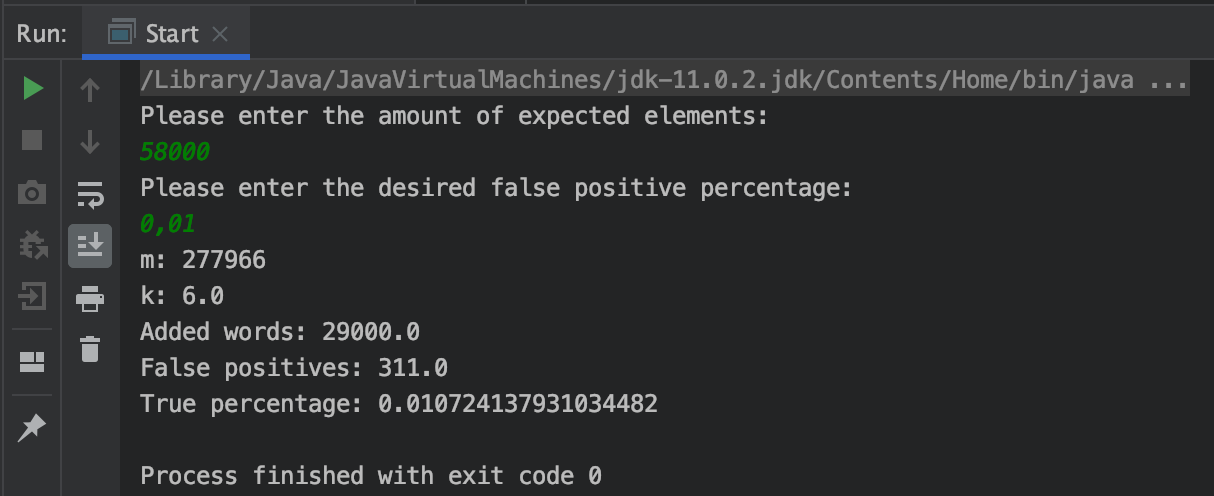
\includegraphics[width=10cm]{image/Result.png}



\end{document}
